\mchapter{مفاهیم و کار های انجام شده}
پژوهش‌های انجام شده در زمینه تخلیه‌ی پردازش را می‌توان بر حسب «ویژگی‌های محیط مسئله» و همینطور «الگوریتم استفاده شده برای حل مسئله» دسته‌بندی کرد. در این فصل ابتدا به معرفی این ویژگی‌ها و الگوریتم‌ها می‌پردازیم و سپس برخی از مقالاتی که ارتباط نزدیکی با \CurrentProject دارند را معرفی می‌کنیم.

\section[مفاهیم اولیه]{مفاهیم اولیه}
\subsection {\lr{Code Smell}}
بوی کد در برنامه‌نویسی کامپیوتر، به ویژگی‌ها یا نشانه‌هایی در کد یک برنامه که حاکی از وجود مشکلاتی در عمق برنامه باشند، بوی کد گفته می‌شود.تعیین اینکه چه چیزی کد بو محسوب می‌شود یا نه، وابسته به فرد توسعه‌دهنده، زبان برنامه‌نویسی و متد توسعه می‌باشد.
یک شیوه برای نگاه به کد بو در نظر گرفتن اصول و کیفیت طراحی است و بوهای کد ساختارهایی مشخص در کد هستند که اصول پایه‌ای برنامه‌نویسی را به گونه‌ای نقض کرده‌اند و کیفیت طراحی را پایین آورده‌اند.

در واقع بوهای بد کد خطا محسوب نمی‌شوند به این معنا که مانع از کارکرد صحیح برنامه نمی‌شوند. آنها ضعف‌هایی در طراحی را نمایان می‌کنند که باعث کند شدن روند توسعه هستند یا ریسک ایجاد خطاها یا خرابی در آینده را افزایش می‌دهند.

معمولاً مشکل عمیق‌تری که بوی بد کد به آن اشاره دارد توسط یک دور بازخورد کوتاه نمایان می‌شود، زمانی که کد در قدم‌هایی کوتاه و کنترل‌شده بازسازی می‌شود و نتیجه برای یافتن بوی بد و بازسازی دوباره، ارزیابی می‌شود. از دید یک برنامه‌نویس که مسئول بازسازی کد است، بوی بد راهنمای او در فرایند بازسازی و انتخاب تکنیک بازسازی است.\cite{whatiscodesmell}
\subsection {\lr{AST}}
درخت نحو انتزاعی نمایش درختی از ساختار نحوی انتزاعی متن و اغلب کد منبع نوشته شده به زبان رسمی است.هر گره درخت نشان‌دهنده یک ساختار در متن است.
انتزاعی بودن نحو به این معناست که تمام جزئیات ظاهر شده در نحو واقعی را نشان نمی‌دهد، بلکه فقط جزئیات ساختاری یا مرتبط با محتوا را نشان می‌دهد.این امر درختان نحو انتزاعی را از درختان نحو انضمامی که به طور سنتی درختان تجزیه نامیده می‌شوند، متمایز می‌کند. درختان تجزیه معمولاً توسط یک تجزیه‌کننده در طول فرایند ترجمه و کامپایل کد منبع ساخته می‌شوند. پس از ساخته شدن، اطلاعات اضافی با پردازش بعدی، به عنوان مثال، تجزیه و تحلیل زمینه‌ای به \lr{AST} اضافه می‌شود.
\begin{figure}[H]
	\centering
	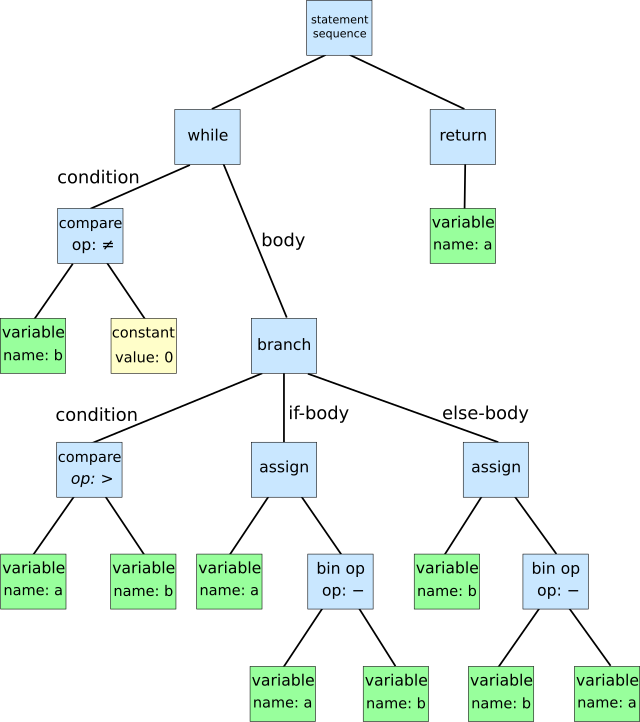
\includegraphics[width=0.7\textwidth]{figures/AST.png}
	\caption{مثالی از درخت نحو انتزاعی }
	\label{fig:AST}
\end{figure}
\clearpage

یک درخت نحو انتزاعی  معمولا به دلیل مراحل متوالی تجزیه و تحلیل توسط کامپایلر، حاوی اطلاعات اضافی در مورد برنامه است.درخت نحو انتزاعی ها به دلیل ماهیت ذاتی زبان‌های برنامه‌نویسی و مستندات آن‌ها مورد نیاز هستند. زبان‌ها معمولاً به طور ذاتی مبهم هستند. برای جلوگیری از این ابهام، زبان‌های برنامه‌نویسی اغلب به عنوان گرامر مستقل از متن \lr{CFG} مشخص می‌شوند. با این حال، اغلب جنبه‌هایی از زبان‌های برنامه‌نویسی وجود دارند که بخشی از زبان هستند و در مشخصات آن مستند شده‌اند ولی یک گرامر مستقل از متن  نمی‌تواند آن‌ها را بیان کند. این‌ها جزییاتی هستند که برای تعیین اعتبار و رفتارشان نیاز به یک زمینه دارند.حتی اگر یک زبان دارای مجموعه‌ای از انواع از پیش تعریف‌شده باشد، اعمال استفاده مناسب اغلب به زمینه‌ای نیاز دارد.

درخت نحو انتزاعی به شدت در طول تجزیه و تحلیل معنایی که در آن کامپایلر استفاده صحیح از عناصر برنامه و زبان را بررسی می‌کند، استفاده می‌شود. کامپایلر همچنین جداول نماد را بر اساس  \lr{AST} در طول تجزیه و تحلیل معنایی تولید می‌کند. پیمایش کامل درخت اجازه می‌دهد تا صحت برنامه تأیید شود.
پس از تأیید صحت،  \lr{AST} به عنوان پایه‌ای برای تولید کد عمل می کند.  \lr{AST} اغلب برای تولید یک نمایش میانی  \lr{IR} که گاهی اوقات زبان میانی نامیده می‌شود، برای تولید کد استفاده می‌شود.
\cite{ast}
\subsection {\lr{RNN}}
راه حل اولیه پژوهشگران برای پردازش متن، ارائه مدل شبکه عصبی بازگشتی بوده است.  این مدل در واقع با
استفاده از ساختار بازگشتی بودن خود راه حلی برای وابسته بودن ورودی ها در اثر زمان پیدا کرده است. به طوری که
مدل های دیگر شبکه ی عصبی داده ها را به صورت ترتیبی نمی بینند و خروجی نورون ها به یکدیگر وابسته نیستند.
\begin{figure}[H]
	\centering
	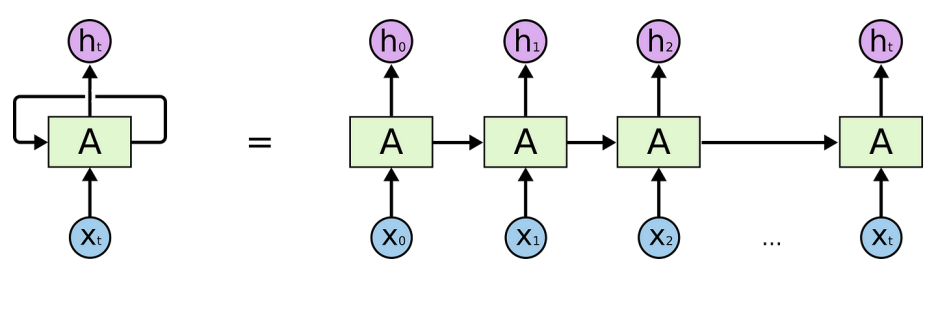
\includegraphics[width=0.7\textwidth]{figures/RNN.png}
	\caption{معماری شبکه عصبی بازگشتی}
	\label{fig:RNN}
\end{figure}

در شکل \ref{fig:RNN} مشاهده می شود که هر ورودی در خروجی های بعدی خود تاثیر می گذارد که اینگونه حتی آخرین نورون
هم قادر به اصلاح اولین نورون از طریق تابع ضرر و محاسبه گرادیان می باشد.
\cite{SHERSTINSKY2020132306}
\subsection{\lr{LSTM}}
به مرور زمان و با آموزش مدل های شبکه ی بازگشتی، محققان شاهد مشکل محوشدگی و انفجار گرادیان در این نوع
شبکه های عصبی بوده اند. یعنی به مرور زمان دچار فراموشی داده های قبلی و در نتیجه ساختار کلی متن را فراموش
می کردند.
سپس با ارائه مدل حافظه طولانی کوتاه مدت \lr{(LSTM)} توانستند بر این مشکل غلبه کنند به طوری که با تعریف دروازه های
ورودی، فراموشی و خروجی داده های مورد نیاز را نگه می داشتند و داده های غیرقابل استفاده را از درون حافظه پاک
می کردند

\begin{figure}[H]
	\centering
	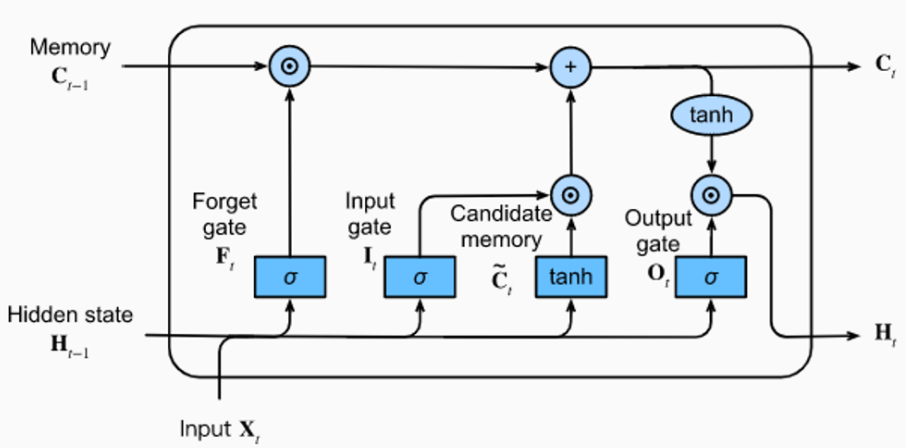
\includegraphics[width=0.7\textwidth]{figures/LSTM.png}
	\caption{معماری شبکه عصبی \lr{(LSTM)}}
	\label{fig:LSTM}
\end{figure}

شکل  \ref{fig:LSTM} به خوبی ساختار درون هر لایه شبکه ی \lr{(LSTM)} را نشان می دهد که در واقع نحوه ی دروازه ها را مشخص
می کند. به واسطه تعریف دروازه های مجزا این شبکه چهار برابر شبکه ی عصبی بازگشتی ساده پارامتر دارد و در نتیجه از
نظر محساباتی چهار برابر کندتر از مدل های شبکه ی عصبی بازگشتی می باشد.
\cite{LINDEMANN2021650}

\subsection{\lr{Attention}}
مدل \lr{(LSTM)} ارائه شده همچنان دچار فراموشی هایی به مرور زمان می شد و نمی توانست یک دنباله با طول بسیار زیاد را
به خاطر بسپارد و همچنان مشکلی محوشدن گرادیان مشاهده می شد. برای برطرف کردن مشکل ذکرشده پژوهشگران به ایده ی استفاده کردن از سازوکار توجه رسیدند که به قدر خوبی تمام مشکلاتی که تا کنون مطرح شد را حل می کرد.
\begin{figure}[H]
	\centering
	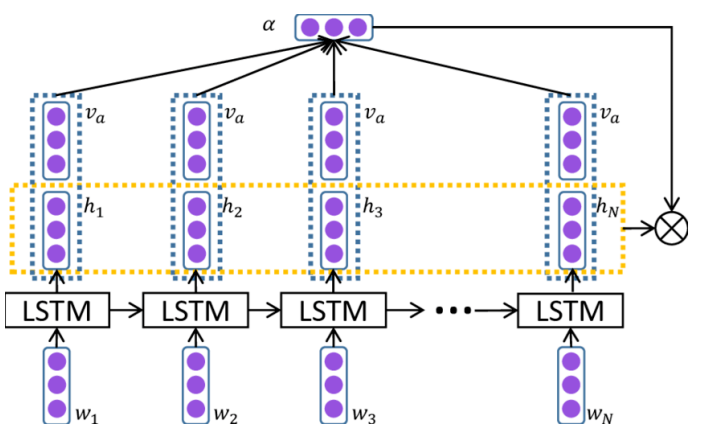
\includegraphics[width=0.7\textwidth]{figures/Attention.png}
	\caption{معماری شبکه عصبی \lr{(Attention)}}
	\label{fig:Attention}
\end{figure}
شکل  \ref{fig:Attention} نشان می دهد که در پردازش هر ورودی، آن لایه می تواند به کل بخش های ورودی توجه کند و با استفاده
از میانگین گیری، مقادیر هر کدام را به نحوی استفاده کند.
\cite{vaswani2017attention}

\subsection{\lr{Transformer}}	
در جدیدترین پژوهش، مدل های ترنسفورمر مطرح شده اند که علم پردازش زبان های طبیعی را متحول کردند. آن ها در
مقاله ی خود ساختاری جدید را معرفی کردند که دیگر ساختار این مدل ها بر پایه شبکه های عصبی بازگشتی نمی باشند.
راه حل نوینی برای بردارهای وابسته به متن ارائه کرده اند که در 
نویسندگان این مقاله با ارائه سازوکار توجه به خود
واقع به این معناست اگر دو کلمه ی هم شکل با معنای متفاوت درون متن قرار بگیرند، این سازوکار متوجه تفاوت این دو کلمه
خواهد شد. آن ها همچنین فرآیند وابسته بودن هر بخش در شبکه های عصبی بازگشتی که منجر به کند بودن آن می شد را
با استفاده از مدل جدید خود کاملا به طور موازی درآوردند که بسیار به کار سرعت می بخشید.
قدم بزرگ دیگر این ساختار، آموزش دیدن مدل های کارآمدی می باشند که در واقع با استفاده
از این مدل ها که بر روی حجم بسیار عظیمی از متن ها آموزش دیده اند، می توانیم از وزن های آموزش دیده ی آن ها در مسائل مختلف استفاده کنیم و مدل‌ها را برای انجام وظایف جدید بدون نیاز به آموزش دوباره از ابتدا به کار بگیریم. این ویژگی به‌ویژه در مواقعی که داده‌های آموزشی محدود هستند، بسیار مفید است. به عنوان مثال، مدل‌های ترنسفورمر که بر روی مقادیر عظیمی از داده‌های عمومی آموزش دیده‌اند، می‌توانند با تنظیمات اندک و استفاده از وزن‌های یادگیری‌شده، به سرعت به مسائل خاصی مانند ترجمه، خلاصه‌سازی متن، یا پاسخ به سوالات پاسخ دهند.
\\
این مدل‌ها همچنین به دلیل ساختار مقیاس‌پذیری که دارند، امکان پردازش موازی را فراهم می‌کنند که این امر منجر به کاهش زمان آموزش و پیش‌بینی می‌شود. علاوه بر این، مدل‌های ترنسفورمر به دلیل حذف محدودیت‌های مربوط به وابستگی‌های طولانی‌مدت در متن، قادر به درک بهتر و عمیق‌تری از توالی‌های طولانی هستند.
\\
مدل‌های ترنسفورمر، از جمله معروف‌ترین آن‌ها یعنی \lr{BERT}، \lr{GPT} و \lr{T5}، به عنوان پایه‌ای برای بسیاری از کاربردهای عملی در پردازش زبان طبیعی مورد استفاده قرار گرفته‌اند. این مدل‌ها توانسته‌اند در بسیاری از معیارهای استاندارد، عملکردی بهتر از مدل‌های پیشین ارائه دهند و در واقع، انقلابی در این حوزه به وجود آورده‌اند.
\\
در نهایت، ترنسفورمرها با ارائه رویکردی جدید به پردازش زبان طبیعی، امکان توسعه سیستم‌های هوشمندتر و کارآمدتر را فراهم کرده‌اند که می‌توانند در طیف وسیعی از کاربردها از جمله ترجمه ماشینی، تولید متن، تحلیل احساسات و بسیاری دیگر به کار گرفته شوند. این مدل‌ها به دلیل انعطاف‌پذیری و قدرت پیش‌بینی بالای خود، همچنان در حال پیشرفت و بهبود هستند و تحقیقات بیشتری در این زمینه در حال انجام است تا از پتانسیل کامل آن‌ها بهره‌برداری شود.
\cite{vaswani2017attention}

\begin{figure}[H]
	\centering
	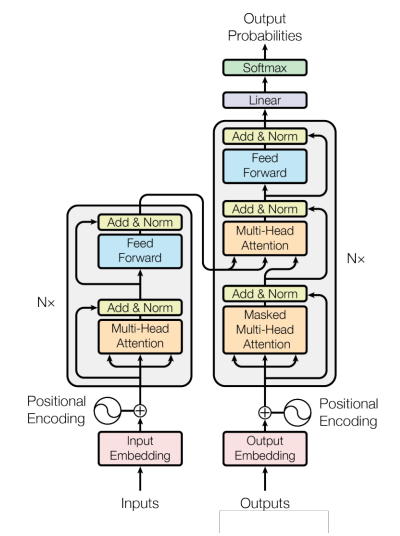
\includegraphics[width=0.5\textwidth]{figures/Transformer.png}
	\caption{معماری \lr{(Transformer)}}
	\label{fig:Transformer}
\end{figure}
شکل \ref{fig:Transformer} معماری مدل \lr{Transformer} را نشان میدهد که لایه هر مرحله چگونه است.

\subsection{\lr{LLaMA}}
مدل \lr{LLaMA} به دلیل استفاده از مکانیسم توجه، قابلیت پردازش کارآمد و موازی داده‌های متنی را دارد. در ساختار، مکانیسم خودتوجهی به مدل اجازه می‌دهد تا به تمامی بخش‌های ورودی توجه کند و روابط بین کلمات را درک کند. این امر به مدل امکان می‌دهد وابستگی‌های طولانی‌مدت در متن را شناسایی کند. محاسبات توجه با استفاده از انجام می‌شود که به بهبود پایداری عددی در پردازش داده‌های بزرگ کمک می‌کند.
\begin{figure}[H]
	\centering
	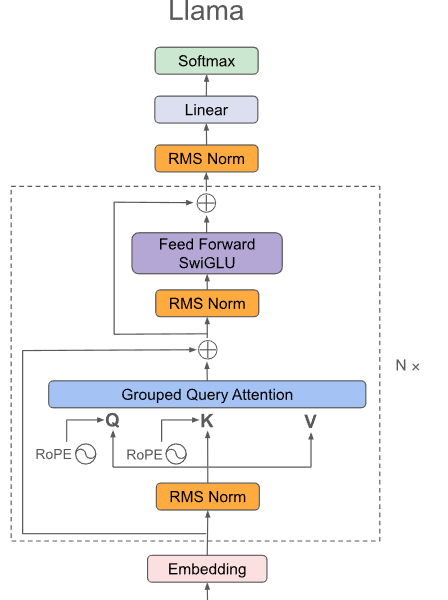
\includegraphics[width=0.5\textwidth]{figures/LLaMA.png}
	\caption{معماری \lr{(LLaMA)}}
	\label{fig:LLaMA}
\end{figure}
شکل \ref{fig:LLaMA} معماری مدل \lr{LLaMA} را نشان میدهد که از لایه‌های متوالی تشکیل شده که شامل بخش کدگذار و کدگشا است. در کاربردهایی مانند ترجمه، هر دو بخش استفاده می‌شوند، اما برای تولید متن معمولاً فقط کدگشا کافی است. هر لایه شامل مکانیزم خودتوجهی و لایه‌های شبکه عصبی کاملاً متصل است. برای تثبیت و تسریع آموزش مدل، از نرمال‌سازی لایه استفاده می‌شود. همچنین، اتصالات باقیمانده به جلوگیری از مشکل کمک می‌کنند و اطلاعات را به‌طور موثرتری در لایه‌های مدل منتقل می‌کنند.
مدل \lr{LLaMA} با اندازه‌های مختلف و تعداد پارامترهای متفاوت عرضه می‌شود، که این امر به کاربران اجازه می‌دهد مدل مناسب را بر اساس نیاز و منابع محاسباتی خود انتخاب کنند. این مدل‌ها به دلیل طراحی بهینه و استفاده از معماری، از کارایی محاسباتی بالایی برخوردارند و قادر به پردازش موازی داده‌ها هستند، که این امر باعث افزایش سرعت و کاهش زمان آموزش می‌شود.
بهبودهای خاص \lr{LLaMA} ممکن است شامل تکنیک‌های کاهش پیچیدگی زمانی و مکانی و استفاده از پیش‌آموزش‌های خاص برای افزایش دقت در وظایف خاص باشد. این مدل‌ها به‌گونه‌ای طراحی شده‌اند که می‌توانند در محیط‌های مختلفی از جمله دستگاه‌های با قدرت محاسباتی محدود اجرا شوند، که این ویژگی آن‌ها را برای کاربردهای صنعتی و تحقیقاتی که نیاز به پردازش سریع و دقیق دارند، بسیار مفید می‌سازد.
در مجموع، \lr{LLaMA} با استفاده از ساختار و بهینه‌سازی‌های مختلف، یک ابزار قدرتمند برای پردازش زبان طبیعی ارائه می‌دهد که می‌تواند در طیف وسیعی از کاربردها مورد استفاده قرار گیرد.\cite{touvron2023llama}

\clearpage
\section[کار های انجام شده با روش های پیشین]{کار های انجام شده با روش های پیشین}
\subsection{سیستم های قانون محور}
سیستم‌های قانون‌محور یا  یکی از رویکردهای اصلی برای تشخیص بوی کد در صنعت نرم‌افزار هستند. این سیستم‌ها بر اساس تعدادی از قوانین یا قواعد برنامه نویسی شده توسط توسعه‌دهندگان عمل می‌کنند. این قواعد معمولاً بر اساس اصول نگارش کد، الگوهای طراحی خوب و استانداردهای برنامه نویسی تعریف شده‌اند.\cite{ruleBased}
\subsubsection{تعریف قوانین}
در این مرحله، توسعه‌دهندگان قوانین مربوط به بوی کد را تعریف می‌کنند. این قوانین ممکن است شامل الگوهای طراحی، اصول نگارش کد، استفاده از متغیرهای مفهومی، اصول  و سایر استانداردهای برنامه نویسی باشند.
\subsubsection{پیاده‌سازی قوانین}
قوانین تعریف شده باید به صورت قابل اجرا در سیستم پیاده‌سازی شوند. این به‌معنای تبدیل قوانین بوی کد به قواعد قابل اجرا توسط سیستم است تا بتواند کد را تحلیل کرده و مشکلات را شناسایی کند.
\subsubsection{تحلیل کد و اعمال تغییرات}
سیستم قوانین و قواعد تعریف شده را بر روی کد منبع اجرا می‌کند. سپس با توجه به این قوانین، بوی کد را تشخیص داده و مشکلات مربوط به کیفیت کد را شناسایی می‌کند. این تحلیل معمولاً شامل اعلام هشدارها، پیشنهادات بهبود و گزارش‌های مرتبط با بوی کد است.
بر اساس نتایج حاصل از تحلیل، توسعه‌دهندگان می‌توانند تغییرات لازم را در کد اعمال کنند تا بهبودهای مورد نیاز را انجام دهند. این شامل اصلاحات نگارشی، بهبودهای ساختاری و سایر تغییراتی است که برای بهبود کیفیت کد لازم است.
\subsection{یادگیری ماشین}
در طول زمان ابزار شناسایی بوی کد نیز پیشنهاد شده است که بیشتر آن‌ها به عنوان مبتنی بر اکتشافی در نظر گرفته می‌شوند.آن‌ها یک فرآیند دو مرحله‌ای را اجرا می‌کنند که در آن ابتدا مجموعه‌ای از متریک‌ها محاسبه می‌شود و سپس برخی آستانه‌ها برای تمایز بین کلاس‌های با بو و بدون بو اعمال می‌شود. این ابزارها از نظر الگوریتم‌های خاص مورد استفاده برای شناسایی بوی کد و متریک‌های بهره‌برداری شده با یکدیگر تفاوت دارند. اگرچه نشان داده شده است که این ابزارها در زمینه دقت توصیه‌ها عملکرد معقولی دارند، ولی کارهای قبلی تعدادی محدودیت مهم را نشان داده‌اند که ممکن است استفاده عملی از این ابزارها را محدود کند. به خصوص، بوهای کدی که توسط ابزارهای موجود شناسایی می‌شوند می‌توانند به صورت ذهنی توسط توسعه‌دهندگان تفسیر شوند. به‌علاوه، توافق بین آن‌ها پایین است. مهم‌تر از همه، بیشتر آن‌ها نیاز به تعیین آستانه‌هایی دارند تا مؤلفه‌های بوی کد را از مؤلفه‌های بدون بوی تمایز بدهند و به طور طبیعی، انتخاب آستانه‌ها به شدت بر دقت آن‌ها تأثیر می‌گذارد.

به دلیل تمامی این دلایل، یک روند جدید به سمت استفاده از تکنیک‌های یادگیری ماشین برای مقابله با این مشکل پیش رفته است. در این سناریو، یک روش نظارت‌شده استفاده می‌شودکه مجموعه‌ای از متغیرهای مستقل برای پیش‌بینی ارزش یک متغیر وابسته (یعنی بوی کد یک کلاس) با استفاده از یک طبقه‌بند یادگیری ماشین به کار می‌روند. مدل می‌تواند با استفاده از مقدار کافی داده‌های موجود از پروژه تحت بررسی، یعنی استراتژی درون‌پروژه‌ای، یا با استفاده از داده‌های پروژه‌های نرم‌افزاری دیگر، یعنی استراتژی بین‌پروژه‌ای، آموزش داده شود. این رویکردها به وضوح از روش‌های مبتنی بر اکتشافی متفاوت هستند، زیرا آن‌ها به طبقه‌بندها برای تمایز بوی کد کلاس‌ها تکیه می‌کنند نه بر آستانه‌های از پیش تعریف‌شده بر روی متریک‌های محاسبه‌شده.\cite{ml}\cite{kaur2017support}

\subsection{یاگیری عمیق}
در حوزه شناسایی بوی کد، یادگیری عمیق به عنوان یک رویکرد نوآورانه و قدرتمند در حال ظهور است. یادگیری عمیق، به ویژه شبکه‌های عصبی عمیق، می‌تواند به طور خودکار ویژگی‌های پیچیده و غیرخطی را از داده‌های ورودی استخراج کند که این امر به بهبود دقت و کارایی در شناسایی بوی کد کمک می‌کند.
\\
یادگیری عمیق، برخلاف روش‌های سنتی یادگیری ماشین که به ویژگی‌های دستی یا از پیش تعریف‌شده متکی هستند، قابلیت یادگیری و استخراج خودکار ویژگی‌ها را دارد. این امر می‌تواند به کاهش وابستگی به آستانه‌های ثابت و بهبود دقت مدل در شناسایی بوی کد کمک کند.
شبکه‌های عصبی عمیق مانند شبکه‌های کانولوشنی یا شبکه‌های بازگشتی به طور خودکار ویژگی‌های سطح بالا و پیچیده را از داده‌های خام استخراج می‌کنند. این فرآیند به مدل اجازه می‌دهد تا روابط پیچیده‌تر و الگوهای غیرخطی را که ممکن است توسط روش‌های سنتی کشف نشود، شناسایی کندود ر یادگیری عمیق، معماری شبکه شامل لایه‌های متعدد (لایه‌های پنهان) است که هر لایه به عنوان یک استخراج‌کننده ویژگی عمل می‌کند. لایه‌های اولیه ویژگی‌های ساده‌تر و لایه‌های عمیق‌تر ویژگی‌های پیچیده‌تر و انتزاعی‌تر را استخراج می‌کنند. یکی از مزایای اصلی یادگیری عمیق این است که نیاز به مهندسی ویژگی دستی را کاهش می‌دهد، چرا که مدل به طور خودکار ویژگی‌های مناسب را از داده‌ها استخراج و یاد می‌گیرد.
\\
مدل‌های یادگیری عمیق نیاز به مقدار زیادی داده برای آموزش دارند تا بتوانند ویژگی‌های مفید را به خوبی یاد بگیرند. می‌توان از تکنیک‌هایی مانند یادگیری انتقالی استفاده کرد که در آن مدل‌های از پیش آموزش‌دیده بر روی مجموعه داده‌های بزرگ‌تر به پروژه‌های خاص تطبیق داده می‌شوند. این روش به خصوص در شرایطی که داده‌های محدود موجود است، مفید است.
\\
ارزیابی مدل‌های یادگیری عمیق نیز مشابه روش‌های سنتی یادگیری ماشین است، اما می‌تواند به دقت بیشتری دست یابد. معیارهایی مانند دقت، فراخوان، و امتیاز \lr{F1} برای ارزیابی مدل‌ها استفاده می‌شوند. همچنین، استفاده از تکنیک‌های اعتبارسنجی متقابل می‌تواند به ارائه ارزیابی دقیق‌تر کمک کند.\cite{liu2019deep}\cite{das2019detecting}

\clearpage
